\documentclass[12pt,openright,oneside,a4paper,english,brazil]{abntex2}

% Pacotes básicos 
\usepackage{lmodern}			% Usa a fonte Latin Modern			
\usepackage[T1]{fontenc}		% Selecao de codigos de fonte.
\usepackage[utf8]{inputenc}		% Codificacao do documento (conversão automática dos acentos)
\usepackage{lastpage}			% Usado pela Ficha catalográfica
\usepackage{indentfirst}		% Indenta o primeiro parágrafo de cada seção.
\usepackage{color}				% Controle das cores
\usepackage{graphicx}			% Inclusão de gráficos
\usepackage{microtype} 			% para melhorias de justificação
\usepackage{amsmath}

\renewcommand\thesubsubsection{}


% CONFIGURAÇÕES DE PACOTES

% Informações de dados para CAPA e FOLHA DE ROSTO
\titulo{Restauração de Imagens de Placas de Veículos Usando Super-resolução}
\autor{David Campos Anchieta}
\local{Belém - PA}
\data{2017}
\orientador{Prof. Dr. Ronaldo de Freitas Zampolo}
\instituicao{%
	Universidade Federal do Pará
	\par
	Instituto de Tecnologia
	\par
	Faculdade de Engenharia da computação e Telecomunicações}
\tipotrabalho{Trabalho de Conclusão de Curso}
% O preambulo deve conter o tipo do trabalho, o objetivo, 
% o nome da instituição e a área de concentração 

% ISSUE: redigir preambulo
\preambulo{ PREÂMBULO }


% Configurações de aparência do PDF final

% alterando o aspecto da cor azul
\definecolor{blue}{RGB}{41,5,195}

% informações do PDF
\makeatletter
\hypersetup{
			%pagebackref=true,
		pdftitle={\@title}, 
		pdfauthor={\@author},
			pdfsubject={\imprimirpreambulo},
			pdfcreator={LaTeX with abnTeX2},
		pdfkeywords={abnt}{latex}{abntex}{abntex2}{trabalho acadêmico}, 
		colorlinks=true,       		% false: boxed links; true: colored links
			linkcolor=blue,          	% color of internal links
			citecolor=blue,        		% color of links to bibliography
			filecolor=magenta,      		% color of file links
		urlcolor=blue,
		bookmarksdepth=4
}
\makeatother

% Espaçamentos entre linhas e parágrafos 
% O tamanho do parágrafo é dado por:
\setlength{\parindent}{1.3cm}

% Controle do espaçamento entre um parágrafo e outro:
\setlength{\parskip}{0.2cm}  % tente também \onelineskip

% compila o indice
\makeindex

% Início do documento
\begin{document}

% Seleciona o idioma do documento (conforme pacotes do babel)
%\selectlanguage{english}
\selectlanguage{brazil}

% Retira espaço extra obsoleto entre as frases.
\frenchspacing 
% ELEMENTOS PRÉ-TEXTUAIS

% Capa
\imprimircapa

% Folha de rosto
\imprimirfolhaderosto

% Inserir folha de aprovação

% Isto é um exemplo de Folha de aprovação, elemento obrigatório da NBR
% 14724/2011 (seção 4.2.1.3). Você pode utilizar este modelo até a aprovação
% do trabalho. Após isso, substitua todo o conteúdo deste arquivo por uma
% imagem da página assinada pela banca com o comando abaixo:
%
% \includepdf{folhadeaprovacao_final.pdf}
%

\begin{folhadeaprovacao}
%ISSUE: folha de aprovação
	\begin{center}
		{\ABNTEXchapterfont\large\imprimirautor}

		\vspace*{\fill}\vspace*{\fill}
		\begin{center}
			\ABNTEXchapterfont\bfseries\Large\imprimirtitulo
		\end{center}
		\vspace*{\fill}
		
		\hspace{.45\textwidth}
		\begin{minipage}{.5\textwidth}
				\imprimirpreambulo
		\end{minipage}%
		\vspace*{\fill}
	 \end{center}
				
	 Trabalho aprovado. \imprimirlocal, 24 de novembro de 2012:

	 \assinatura{\textbf{\imprimirorientador} \\ Orientador} 
	 \assinatura{\textbf{Professor} \\ Convidado 1}
	 \assinatura{\textbf{Professor} \\ Convidado 2}
	 %\assinatura{\textbf{Professor} \\ Convidado 3}
	 %\assinatura{\textbf{Professor} \\ Convidado 4}
			
	 \begin{center}
		\vspace*{0.5cm}
		{\large\imprimirlocal}
		\par
		{\large\imprimirdata}
		\vspace*{1cm}
	\end{center}
	
\end{folhadeaprovacao}

% Dedicatória
\begin{dedicatoria}
%ISSUE: dedicatória
	 \vspace*{\fill}
	 \centering
	 \noindent
	 \textit{ DEDICATÓRIA} \vspace*{\fill}
\end{dedicatoria}

% Agradecimentos
\begin{agradecimentos}
%ISSUE: agradecimentos


\end{agradecimentos}

% Epígrafe
\begin{epigrafe}
%ISSUE: epígrafe
		\vspace*{\fill}
	\begin{flushright}
		\textit{O que as suas mãos tiverem que fazer,\\
		que o façam com toda a sua força,\\
		pois na sepultura, para onde você vai,\\
		não há atividade nem planejamento,\\
		não há conhecimento nem sabedoria.\\
Eclesiastes 9:10}
	\end{flushright}
\end{epigrafe}

% RESUMOS

% resumo em português
\setlength{\absparsep}{18pt} % ajusta o espaçamento dos parágrafos do resumo
\begin{resumo}
%ISSUE: resumo pt

\end{resumo}

% resumo em inglês
\begin{resumo}[Abstract]
%ISSUE: resumo en
 \begin{otherlanguage*}{english}
	This is the english abstract.

	\vspace{\onelineskip}
 
	\noindent 
	\textbf{Keywords}: latex. abntex. text editoration.
 \end{otherlanguage*}
\end{resumo}


% inserir lista de ilustrações
\pdfbookmark[0]{\listfigurename}{lof}
\listoffigures*
\cleardoublepage
% ---

% ---
% inserir lista de tabelas
% ---
\pdfbookmark[0]{\listtablename}{lot}
\listoftables*
\cleardoublepage
% ---

% ---
% inserir lista de abreviaturas e siglas
% ---
\begin{siglas}
	\item[SR] Super-resolução
	\item[HR] \emph{High resolution}
	\item[LR] \emph{Low resolution}
	\item[PDF] \emph{Probalility density function}

\end{siglas}
% ---

% ---
% inserir lista de símbolos
% ---
\begin{simbolos}
%ISSUE: lista de símbolos
	\item[$ \mathbf{x} $] Vetor com os dados da imagem de alta resolução.
	\item[$ \mathbf{y}_k $] Vetor da imagem de alta resolução de número k.
	\item[$ K $] Número de imagens de baixa resolução.
	\item[$ N $] Número de pontos na imagem de alta resolução.
    \item[$ M $] Número de pontos na imagem de baixa resolução.
    \item[$ \mathbf{W}^{(k)}$] Matriz de degradação da imagem de número k.
    \item[$ \gamma $] Largura da função de espalhamento de ponto.
    \item[$ \theta_k $] Ângulo de rotação da imagem de número k.
    \item[$ \mathbf{s}_k $] Vetor com deslocamento bidimensional da imagem de baixa resolução de número k.
    \item[$ \mathbf{Z}_x $] Matriz de covariância da distribuição a priori de $\mathbf{x}$.
    \item[$ \mathbf{\Sigma}$] Matriz de covariância da distibuição a posteriori de $\mathbf{x}$ condicionada aos parâmetros de degradação e conjunto de todos os $\mathbf{y}^{(k)}$.
    \item[$ \boldsymbol{\mu} $] Vetor média da distibuição a posteriori de $\mathbf{x}$ condicionada aos parâmetros de degradação e conjunto de todos os $\mathbf{y}^{(k)}$.
    \item[$ \beta $] Inverso da variância do ruído.
    \item[$ | \cdot | $] Determinante de matriz.
    \item[$\| \cdot \|$] Norma de um vetor.
    
\end{simbolos}
% ---

% ---
% inserir o sumario
% ---
\pdfbookmark[0]{\contentsname}{toc}
\tableofcontents*
\cleardoublepage
% ---



% ----------------------------------------------------------
% ELEMENTOS TEXTUAIS
% ----------------------------------------------------------
\textual

% ----------------------------------------------------------
% Introdução (exemplo de capítulo sem numeração, mas presente no Sumário)
% ----------------------------------------------------------
\chapter[Introdução]{Introdução}
\addcontentsline{toc}{chapter}{Introdução}
% ----------------------------------------------------------
%ISSUE: introdução

% CONTEXTUALIZAÇÃO: ONDE MEU PROBLEMA APARECE?
A disponibilidade de imagens de alta resolução é uma vantagem para a execução de qualquer trabalho que envolva a captação e interpretação de informações através de imagens digitais.
Como exemplo disso podemos citar as imagens médicas, nas quais quanto melhor a qualidade da imagem, mais fácil é diferenciar as estruturas retratadas afim de diagnosticar doenças.
Também há o caso dos sistemas de vigilância, onde quanto melhor a resolução espacial da imagem, mais viável se torna a identificação de veículos e criminosos.

% DELIMITAÇÃO: QUE PROBLEMA ESTOU RESOLVENDO?
Hoje em dia, com as frequentes ameaças à segurança das pessoas em diversos lugares do mundo, os cidadãos sentem a necessidade de investir na própria segurança privada para proteger a si mesmos e seus patrimônios.
Por causa dessa necessidade, houve uma popularização de sistemas de vigilância monitoramento.
As câmeras de segurança já são tão onipresentes em grandes cidades que é praticamente impossível que um cidadão comum saia à rua e não tenha a sua imagem gravada por pelo menos uma delas.

No entanto, apesar da presença geral dos sistemas de vigilância, a maioria dos equipamentos utilizados é de baixa qualidade, o que se reflete nas imagens captadas por eles.
A consequência disso é que muitas vezes as câmeras de monitoramento registram cenas de crimes,
mas as imagens deterioradas nem sempre ajudam a trazer à luz informações importantes, como o rosto de um criminoso ou a placa de um carro, por exemplo.

Não obstante, mesmo com necessidade evidente de se melhorar a qualidade das imagens geradas por sistemas de vigilância,
também há o dilema constante entre aumentar a qualidade das imagens registradas e o custo de implementar manter o sistema de monitoramento funcionando.
Quanto melhor a qualidade da imagem, maior é o custo do equipamento e mais capacidade de armazenamento será necessária para guardar uma quantidade útil de todas as imagens gravadas.


% SOLUÇÕES: O QUE JÁ EXISTE QUE RESOLVE ESTE PROBLEMA?
Face ao dilema das imagens geradas por sistemas de vigilância,
a melhor solução a curto prazo seria aprimorar as imagens que estão sendo geradas pelas câmeras de vigilância que já temos hoje.
Esse aprimoramento seria feito através de restauração de imagens digitais.

A demanda pelo desenvolvimento de técnicas de restauração de imagens ganhou força no fim da década de 1950, quando a sua principal aplicação era na área de imagens astronômicas.
Naquele contexto, era necessário restaurar as primeiras imagens recebidas de sondas e satélites artificiais que sofriam degradações próprias do ambiente onde esses objetos trabalhavam.

Após tantos anos, a restauração de imagens digitais continua tendo sua importância na astronomia, mas também é uma ferramenta para outras áreas como medicina, mídia e ciências forenses \cite{banham1997digital}.

% SOLUÇÃO ESCOLHIDA: O QUE ELA É E COMO FUNCIONA?
Este trabalho descreve a implementação e teste de um método de restauração de imagens de placas de veículos usando super-resolução bayesiana.
O método utilizado foi apresentado por Michael Tipping em \cite{tipping2003bayesian}.
Em resumo, o algorítimo apresentado define um modelo de observação no qual as degradações sofridas pela imagem durante o processo de aquisição são parametrizadas.
Então são usadas inferências bayesianas para estimar os parâmetros de degradação a partir das imagens de baixa resolução, para então estimar a imagem de alta resolução a partir destes parâmetros.

% VANTAGENS: POR QUE ESTA SOLUÇÃO E NÃO AS OUTRAS?
Esta solução foi escolhida devido à adequação do algorítimo à aplicação desejada, que é a restauração de uma imagem de placa de veículo a partir de várias imagens degradadas, como os quadros de um vídeo de câmera de vigilância.
Também vale destacar a relativa simplicidade de implementação do método escolhido, o qual também possibilita ajustes afim de reduzir seu custo computacional.

% ESTRUTURA: O QUE TEM NOS CAPÍTULOS SEGUINTES?

\chapter{Restauração de Imagens Usando Super-resolução}
\section{Introdução}
Entende-se por Super-resolução o processo de obtenção de uma ou mais imagens de alta resolução a partir de uma ou mais imagens de baixa resolução.
Técnicas de super-resolução são pesquisadas desde os anos 1970 e têm despertado um grande interesse de estudo nas últimas décadas.
As aplicações de técnicas de SR são diversas e incluem aprimoramentos de imagens médicas, de imagens de rosto, de texto e impressões digitais \cite{nasrollahi2014super}.

Vale esclarecer que, neste trabalho, a palavra \textit{resolução} se refere à resolução espacial de uma imagem, a qual mede a densidade de pontos por unidade de área em uma imagem \cite{zibetti2007super}.

Este capítulo fará uma breve síntese do histórico das técnicas de super-resolução e seus principais exemplares.

\section{Modelo de Observação}
\label{sec:obsmodel}

Definir um modelo de observação que relacione a imagem de alta resolução às imagens de baixa resolução observadas é fundamental para o desenvolvimento de qualquer técnica de super-resolução.

O modelo de observação deste trabalho simula cinco tipos de alteração aplicadas por sistemas de aquisição de imagens, a saber: rotação, deslocamento, espalhamento de ponto, subamostragem e ruído.
Este modelo de observação é descrito tanto em \cite{tipping2003bayesian} quanto em outros trabalhos relacionados \cite{pickup2007bayesian, Capel01a}.

As alterações de deslocamento linear e rotação tentam simular um possível movimento aleatório da câmera em relação ao objeto.
A transformação de espalhamento de ponto simula um efeito de desfoque causado por um possível desajuste nos aspectos ópticos da câmera.
A subamostragem representa a perda de resolução espacial aplicada à imagem captada por um sensor CMOS ou CCD, por exemplo.
que seria menor do que a necessária para registrar os dados da imagem acima da taxa de Nyquist.

Pela conveniência do modelo de observação, a imagem de alta resolução de dimensões $m \times n$ é representada por um vetor coluna $\mathbf{x} = [x_1, x_2, ... , x_{N-1}, x_N]^T$ onde $N ={} m \times n$. Ou seja, os valores dos pixels da imagem são rearranjados em um vetor de comprimento $N$.

Sabendo disso, a relação entre uma imagem de alta resolução $\mathbf{x}$ e uma imagem degradada $\mathbf{y}^{(k)}$ é resumida em (\ref{eq:degradation}). Onde $k = 1,2,...,K$; sendo $K$ o número total de quadros obtidos a partir da cena de alta resolução $\mathbf{x}$.

\begin{equation}
	\label{eq:degradation}
	\mathbf{y}^{(k)} = \mathbf{W}^{(k)}\mathbf{x} + \mathbf{n}^{(k)}
\end{equation}

O ruído, representado por $\mathbf{n}$ é um vetor de variáveis aleatórias Gaussianas independentes de média zero e variância $1/\beta$.

A matriz de sistema $\mathbf{W}$ aplica as transformações de rotação, deslocamento, subamostragem e espalhamento de ponto ao ser multiplicada pela imagem de alta resolução $\mathbf{x}$.
Pelas propriedades da multiplicação de matrizes, é natural que as dimensões da matriz do sistema sejam $M \times N$; onde $M$ é o número de pixels da imagem resultante.
Também se espera que $N \gg M$.

A matriz $\mathbf{W}$ depende de três parâmetros de transformação: a largura da função de espalhamento de ponto $\gamma$, um ângulo de rotação $\theta$ e um vetor de deslocamento linear $\mathbf{s}$.
Os elementos da matriz são dados por (\ref{eq:wmatrix}) com a função de espalhamento de ponto descrita em (\ref{eq:psf}) enquanto os parágrafos seguintes demonstram como as demais transformações são incorporadas à matriz de sistema.

\begin{gather}
	\label{eq:wmatrix}
	W^{(k)}_{ji} = \widetilde{W}^{(k)}_{ji} / \sum_{i'} \widetilde{W}^{(k)}_{ji} \\
	\label{eq:psf}
	\widetilde{W}^{(k)}_{ji} = \exp \left\{- \frac{\|\mathbf{v}_i - \mathbf{u}^{(k)}_j\|^2}{\gamma^2} \right\}
\end{gather}

Os vetores $\mathbf{u}^{(k)}_j$ representam o centro da função de espalhamento de ponto e é descrito em (\ref{eq:psfcenter}).
Caso não houvesse espalhamento de ponto, as coordenadas $\{\mathbf{u}_1, \mathbf{u}_2,\mathbf{u}_3,..., \mathbf{u}_M\}$ seriam os pontos de amostragem da imagem de baixa resolução na imagem de alta resolução.
A Figura \ref{fig:transformations} mostra como se dá o processo de subamostragem e outras transformações bidimensionais.

O efeito da transformação de espalhamento da função de espalhamento de ponto é o mesmo que o de realizar uma convolução da imagem com uma função Gaussiana bidimensional como a mostrada na Figura \ref{fig:psfplot}.
O efeito da transformação é semelhante ao de um desfoque lente, como mostrado na Figura \ref{fig:psfexample}.


\begin{figure}[h]
	\centering
	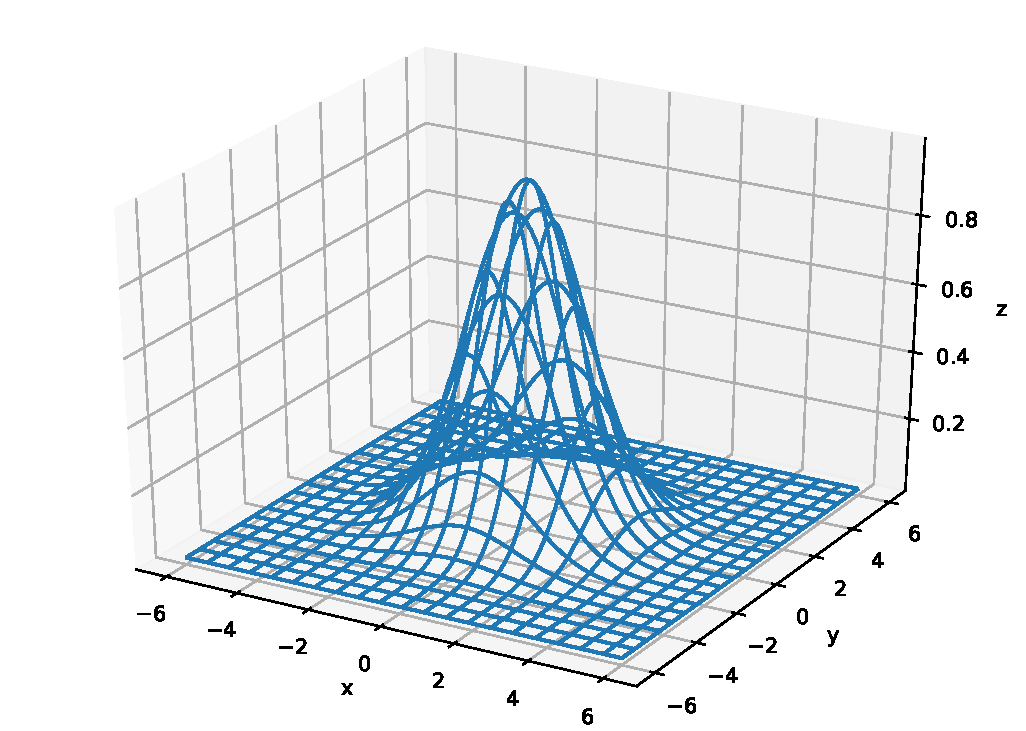
\includegraphics[width = 0.7\textwidth]{./figures/psf1.pdf}
	\caption{Exemplo de gráfico de uma função de espalhamento de ponto com $\gamma = 2$ centrada em $[0,0]$.}
	\label{fig:psfplot}
\end{figure}

\begin{figure}
	\centering
	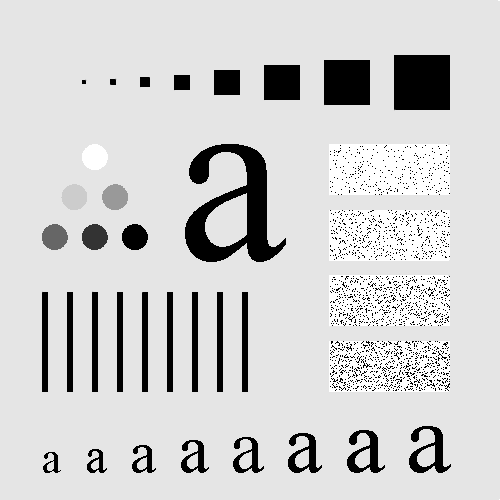
\includegraphics[width = 0.25\textwidth]{./figures/psfexample0.png}
	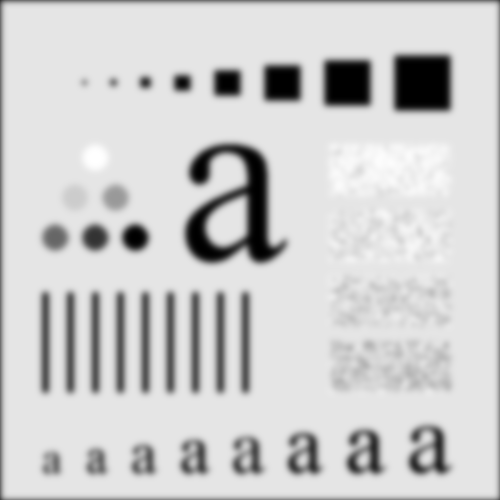
\includegraphics[width = 0.25\textwidth]{./figures/psfexample1.png}
	\caption{Exemplo de convolução de uma imagem com uma função de espalhamento de ponto com $\gamma = 10$.}
	\label{fig:psfexample}
\end{figure}

\begin{equation}
	\label{eq:psfcenter}
	\mathbf{u}^{(k)}_j = \mathbf{R}^{(k)}(\mathbf{v}_j-\mathbf{\overline{v}})+\mathbf{\overline{v}}+\mathbf{s}_k
\end{equation}

\begin{equation}
	\mathbf{R}^{(k)} = 
	\begin{pmatrix}
		\cos \theta_k & \sin \theta_k \\
		- \sin \theta_k & \cos \theta_k
	\end{pmatrix}
\end{equation}

\begin{figure}
	\centering
	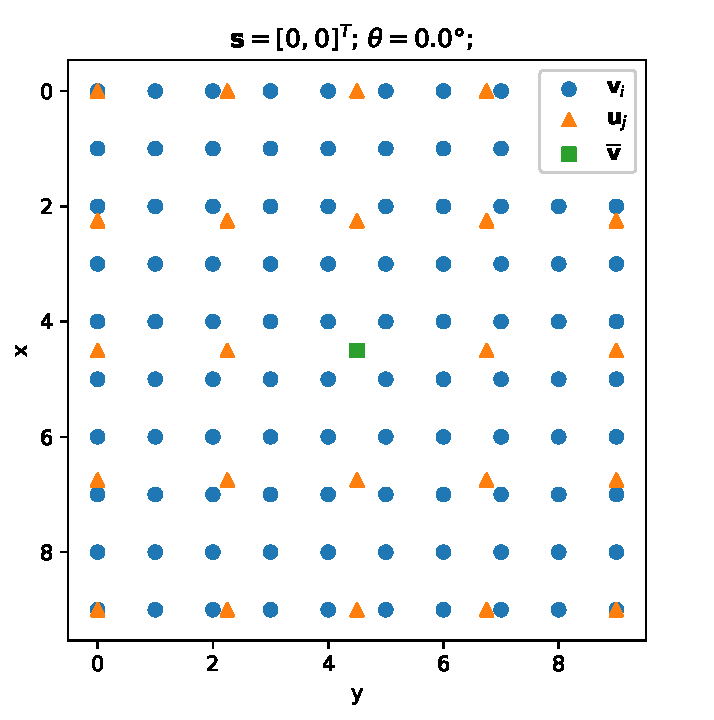
\includegraphics[width=0.3\textwidth]{./figures/transform1.pdf}
	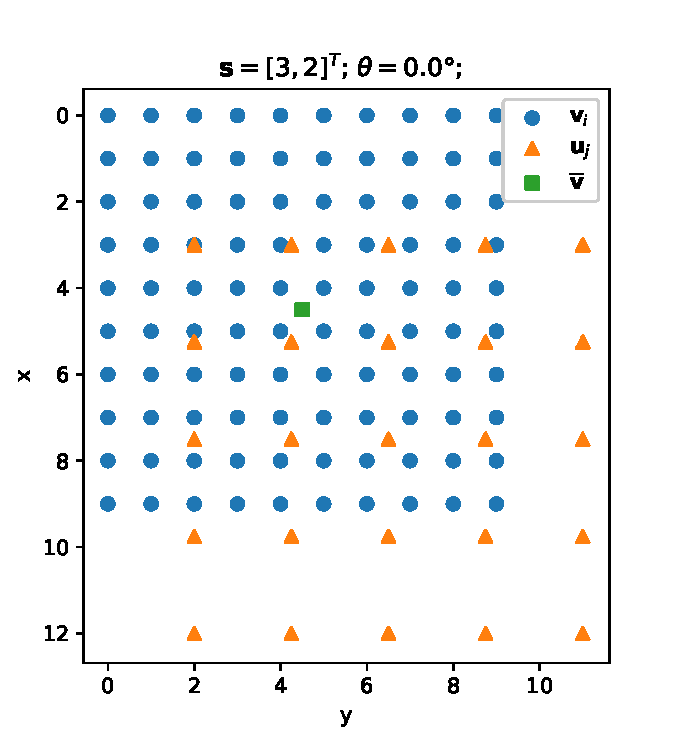
\includegraphics[width=0.3\textwidth]{./figures/transform2.pdf}
	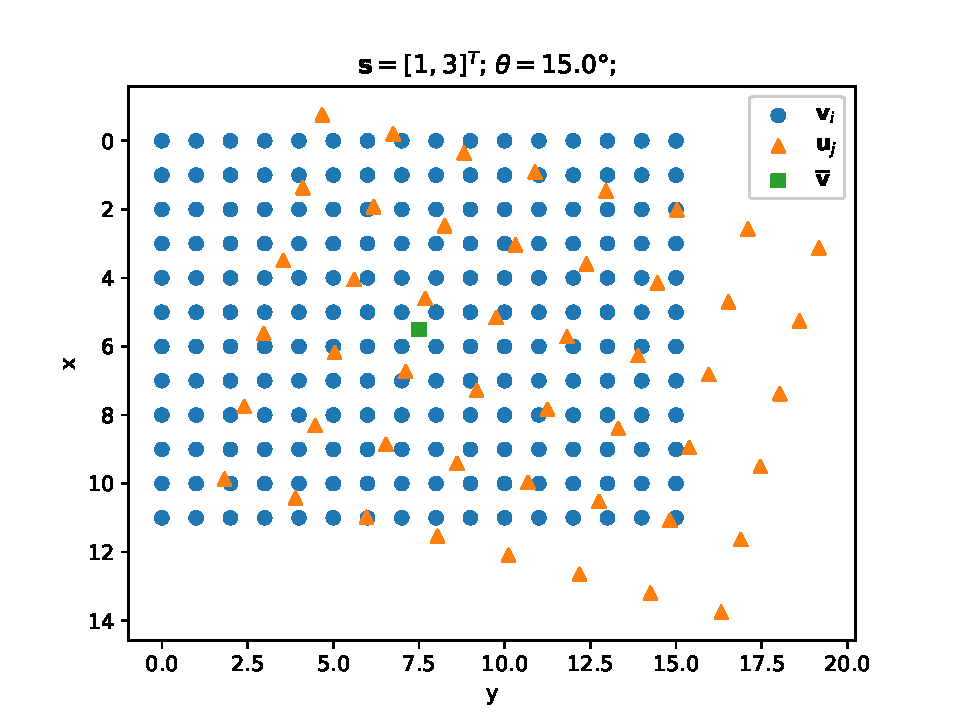
\includegraphics[width=0.3\textwidth]{./figures/transform3.pdf}
	\caption{Visualização das transformações de subamostragem, deslocamento linear e rotação.}
	\label{fig:transformations}
\end{figure}


\section{Apreciação dos Métodos de Super-resolução} 
\subsection{Domínio da Frequência}

Os primeiros algorítimos de super-resolução desenvolvidos faziam o processamento das imagens no domínio da frequência.
Esse tipo de abordagem tinha a vantagem da simplicidade em sua teoria.
No entanto, as técnicas de super-resolução no domínio da frequência tinham limitações com respeito ao tipo de degradação sofrida pela imagem além da dificuldade de aplicar o conhecimento a priori da imagem de alta resolução no domínio espacial para regularização.
Por estes e outros motivos que a maioria dos algorítimos de super-resolução desenvolvidos até hoje faz o processamento das imagens no domínio espacial \cite{park2003super}.

Os trabalhos de Gerchberg \cite{Gerchberg1974} e Santis e Gori \cite{de1975iterative} foram os primeiros a introduzir técnicas de super-resolução no domínio da frequência.
Sendo que o primeiro método a ter múltiplas imagens como entrada foi desenvolvido por Tsai e Huang em 1994 \cite{nasrollahi2014super}.

% ISSUE: Completar seção domínio da frequência.


\subsection{Domínio Espacial}
A maioria dos algorítmos de super-resolução desenvolvidos faz o processamento de imagem no domínio espacial.
Os tipos de abordagens usadas são bastante diversos, sendo que a mais frequente é a probabilística, na qual o método usado neste trabalho está incluído \cite{nasrollahi2014super}.

\subsubsection{Iterative Back Projections}
% ISSUE: Tentar mudar a formatação de subsubsection

O método \emph{Iterative Back Projection} ou retroprojeção iterativa (tradução do autor) foi proposto pela primeira vez em \cite{irani1991improv}.
Trata-se de um método iterativo que visa minimizar o erro a cada execução.

% ISSUE: Inserir IBP na lista de siglas.

A cada interação do método IBP, uma imagem de alta resolução é estimada.
Então é usado o modelo de observação para gerar um conjunto simulado de imagens de baixa resolução.
Esse conjunto de imagens simuladas é comparado às imagens de baixa resolução obtidas através do sistema de aquisição.
A comparação se dá através do cálculo da diferença (erro) entre os dois conjuntos de imagem.
O método iterativo busca minimizar esse erro afim de recuperar a imagem de alta resolução \cite{park2003super,reis2014metodo}.

% SUGGESTION: Inserir figura do esquema de IBP.
% SUGGESTION: Inserir equaçõ do algoritmo de IBP.

\subsubsection{Métodos de Aprendizado}

\subsubsection{Métodos Probabilísticos}


\chapter{Super Resolução Bayesiana}
\section{Funções de probabilidade a priori e a posteriori}

O método algoritmo por Tipping se vale do método de inferência Bayesiana para obter uma imagem de alta resolução a partir de várias imagens de baixa resolução.
Através de um método de inferência Bayesiana, é possível obter uma estimativa de valores desconhecidos (como a imagem de alta resolução) usando um conhecimento a priori que se tem desses dados e informações que já estão disponíveis(no caso, as imagens de baixa resolução) \cite{therrien2011probability}.

Sabendo disso, há a necessidade de formular uma distribuição a priori que represente as características estatísticas da imagem que pretendemos estimar a partir dos dados.
A distribuição de probabilidade a priori escolhida para a imagem é uma gaussiana como descrita a seguir:

\begin{gather}
	p(\mathbf{x}) = \mathcal{N}(\mathbf{x} | 0, \mathbf{Z}_x) \\ 
	Z_x(i,j) = A \exp \left\{ - \frac{\|\mathbf{v}_i - \mathbf{v}_j \|^2}{r^2} \right\}
\end{gather}

Onde $A$ é uma constante, e $r$ determina o quanto cada ponto da imagem de alta resolução depende dos pontos vizinhos.
Expandindo a função densidade de probabilidade $p(\mathbf{x})$ temos:

\begin{equation}
	p(\mathbf{x}) = \frac{1}{\sqrt{(2\pi)^N \mathbf{Z}_x}}\exp{-\tfrac{1}{2} \mathbf{x}^T \mathbf{Z}_x \mathbf{x}}
\end{equation}

Este tipo de distribuição não é o ideal, visto que se definirmos $r=1$, estaríamos dizendo que a maioria dos valores dos pontos da imagem de de alta resolução estão contidos no intervalo $[-1,1]$, o que não condiz com a realidade.
No entanto, o uso desta distribuição a priori será mantido no desenvolvimento deste trabalho pela conveniência proporcionada pela função de probabilidade Gaussiana, que facilita algumas manipulações -- como aplicação de logaritmos naturais --  utilizadas a seguir.

Ciente da relação entre a imagem original e as imagens de baixa resolução, podemos escrever a probabilidade a posteriori das imagens de baixa resolução como:

\begin{equation}
	\label{eq:posterior0}
	p(\mathbf{y}^{(k)} | \mathbf{x}, \mathbf{s}_k, \theta_k, \gamma) = 
	\left(\frac{\beta}{2\pi}\right)^{M/2}
	\exp \left\{ -\frac{\beta}{2} \| \mathbf{y}^{(k)} - \mathbf{W}^{(k)} \mathbf{x} \|^2 \right\}.
\end{equation}

Note que esta distribuição é condicionada na imagem de alta resolução e nos parâmetros de degradação, dados que são desconhecidos em um situação real.

Podemos usar o Teorema de Bayes para isolar a imagem original $\mathbf{x}$, ao que obtemos:

\begin{gather}
	\label{eq:posteriordist}
	p(\mathbf{x}|\{\mathbf{y}^{(k)},\mathbf{s}_k,\theta_k\}, \gamma) = 
	\frac{p(\mathbf{x})\prod^K_{k=1} p(\mathbf{y}^{(k)}|\mathbf{x},\mathbf{s}_k,\theta_k, \gamma)}
	{p(\{\mathbf{y}^{(k)}\}|\{\mathbf{s}_k,\mathbf{\theta}_k\},\gamma)} \\
	= \mathcal{N}(\boldsymbol{\mu},\mathbf{\Sigma}) \\
	\mathbf{ \Sigma }= \left[\mathbf{Z}^{-1}_x + \beta \left( \sum^K_{k = 1} \mathbf{W}^{(k)^T} \mathbf{W}^{(k)} \right) \right]^{-1} \\
	\boldsymbol{\mu} = \beta \mathbf{ \Sigma } \left( \sum^K_{k=1} \mathbf{W}^{(k)^T}\mathbf{y}^{(k)} \right).
\end{gather}

Esta função de probabilidade já poderia ser utilizada para inferir a imagem de alta resolução.
Para isso, bastaria encontrar o valor de $\mathbf{x}$ que maximiza o numerador em (\ref{eq:posteriordist}). entretanto, isso exigiria saber os valores dos parâmetros de degradação ($\gamma$, $\theta_k$, $\mathbf{\theta}_k$).
Como esses parâmetros não estão disponíveis, eles também terão de ser estimados a partir das imagens de baixa resolução $\mathbf{y}_k$. 

A solução proposta no artigo é marginalizar $\mathbf{x}$ em (\ref{eq:posterior0}) para que ele não seja mais uma variável na função. O resultado disto é a seguinte distribuição:

\begin{align}
	\label{eq:parameter}
	\log p(\mathrm{y}|\{\mathbf{s}_k,\theta_k\}, \gamma) &= -\frac{1}{2}\left[\beta \sum^K_{k=1} \|\mathbf{y}^{(k)} - \mathbf{W}^{(k)}\boldsymbol{\mu}\|
    + \boldsymbol{\mu}^T\mathbf{Z}_x \boldsymbol{\mu} \right. \nonumber \\
    &\qquad \left.\vphantom{\int_t} + \log |\mathbf{Z}_x| - \log{|\Sigma |} - KM \log \beta \right].
\end{align}

Onde y é o conjunto de todas as imagens de baixa resolução $\mathbf{y}_k$.

Em uma situação ideal, a melhor estimativa dos valores dos parâmetros de degradação é a que maximiza a função de verossimilhança em (\ref{eq:parameter}).
Tendo a estimativa desses valores, podemos então usá-los em (\ref{eq:posteriordist}) para procurar pelo vetor $\mathbf{x}$ que maximiza aquela função de verossimilhança.

Um fato que se constatou empiricamente na tentativa de calcular os valores da função de verossimilhança é que as probabilidades são muito pequenas ao ponto de estarem fora do intervalo de precisão de uma variável do tipo ponto flutuante.
Os valores também variam muito pouco ao longo do espaço vetorial de $\mathbf{x}$ o que dificultaria o uso de métodos iterativos para encontrar o ponto de máximo da função.

Para resolver isso, aplicou-se o logaritmo natural à função. Isso resolveu o problema da escala e da variação.
Além disso eliminou os exponenciais e os produtos, facilitando o cálculo do gradiente e Jacobiano da função.

\begin{gather}
	L(\mathbf{x}) = -\frac{1}{2} \left\{ \sum^K_{k=1} \|\mathbf{y}^{(k)} - \mathbf{W}^{(k)} \mathbf{x} \|^2 + \mathbf{x}^T\mathbf{Z}^{-1}_x\mathbf{x} - KM\mathrm{ln}(\beta) - \mathrm{ln}|\mathbf{Z}_x| \right\} \\ 
	L'(\mathbf{x}) =  \sum^K_{k=1}  (\mathbf{y}^{(k)} - \mathbf{W}^{(k)}\mathbf{x})(\mathbf{W}^{(k)})^T  - \frac{1}{2}(\mathbf{Z}^{-1}_x + (\mathbf{Z}^{-1}_x)^T)\mathbf{x}  \\
	L''(\mathbf{x}) =  -\sum^K_{k=1} (\mathbf{W}^{(k)})^T\mathbf{W}^{(k)} - \frac{1}{2}(\mathbf{Z}^{-1}_x - (\mathbf{Z}^{-1}_x)^T)^T
\end{gather}

\chapter{Resultados}
\section{Geração do conjunto de imagens de teste}
As imagens usadas para testar o método de restauração descrito neste trabalho foram geradas artificialmente a partir de uma única imagem usando o modelo de observação descrito na seção \ref{sec:obsmodel}.


\chapter{Conclusão}

% ELEMENTOS PÓS-TEXTUAIS
\postextual

% Referências bibliográficas
\bibliographystyle{plain}
\bibliography{referencias}


\end{document}
